
\documentclass[12pt]{amsart}
\usepackage{listings}
\usepackage{color}
\usepackage{graphicx}
\usepackage{palatino}
\usepackage{tikz}
\usepackage{amssymb}
\usepackage{cite}
\usepackage[colorlinks,linkcolor=red]{hyperref}
\usetikzlibrary{shapes.geometric, arrows}

\definecolor{dkgreen}{rgb}{0,0.6,0}
\definecolor{gray}{rgb}{0.5,0.5,0.5}
\definecolor{mauve}{rgb}{0.58,0,0.82}

\lstset{frame=tb,
  language=Python,
  aboveskip=3mm,
  belowskip=3mm,
  showstringspaces=false,
  columns=flexible,
  basicstyle={\small\ttfamily},
  numbers=none,
  numberstyle=\tiny\color{gray},
  keywordstyle=\color{blue},
  commentstyle=\color{dkgreen},
  stringstyle=\color{mauve},
  breaklines=true,
  breakatwhitespace=true,
  tabsize=3
}
\title{NLP_HW3}
\author{Xuan Wang}
\date{} % delete this line to display the current date

%%% BEGIN DOCUMENT

\begin{document}


\begin{titlepage}

\begin{center}


% Upper part of the page

\textsc{\LARGE University of Rutgers}\\[1.5cm]

\textsc{\Large Assignment 1: Fast Trajectory Planning}\\[0.5cm]


% Author and supervisor
\begin{minipage}{0.4\textwidth}
\begin{flushleft} \large
\emph{Author:}\\
Xuan \textsc{Wang}

Xunjie \textsc{Zhu}
\end{flushleft}
\end{minipage}
\begin{minipage}{0.4\textwidth}
\begin{flushright} \large
\emph{Supervisor:} \\
Abdeslam  \textsc{Boularias}
\end{flushright}
\end{minipage}

\vfill

% Bottom of the page
{\large \today}

\end{center}

\end{titlepage}

%\section*{Part 0}
%For the maze, define a maze class, use \emph{numpy} external library to generate a 2-d 101*101 int array representing the maze. Then use \emph{networkx} library to convert the maze into an undirected graph by adding edges for each pair of adjacency nodes, use \emph{dfs\_preorder\_nodes()} method to find a traverse list by DFS, for each visited node make it blocked of 30\% chance
%\begin{lstlisting}
%self.array = np.zeros((m,n))
%traverselist = list(nx.dfs_preorder_nodes(self.graph,(0,0)))
%p_list = [1,1,1,0,0,0,0,0,0,0]
%traverselist = self.DFS()
%for i in traverselist:
%	self.array[i[0],i[1]] = random.choice(p_list)
%\end{lstlisting}
%The following picture is a visualization implement by scala
%
%
%\newpage
\section*{Problem 4}
(a)Draw the complete game tree


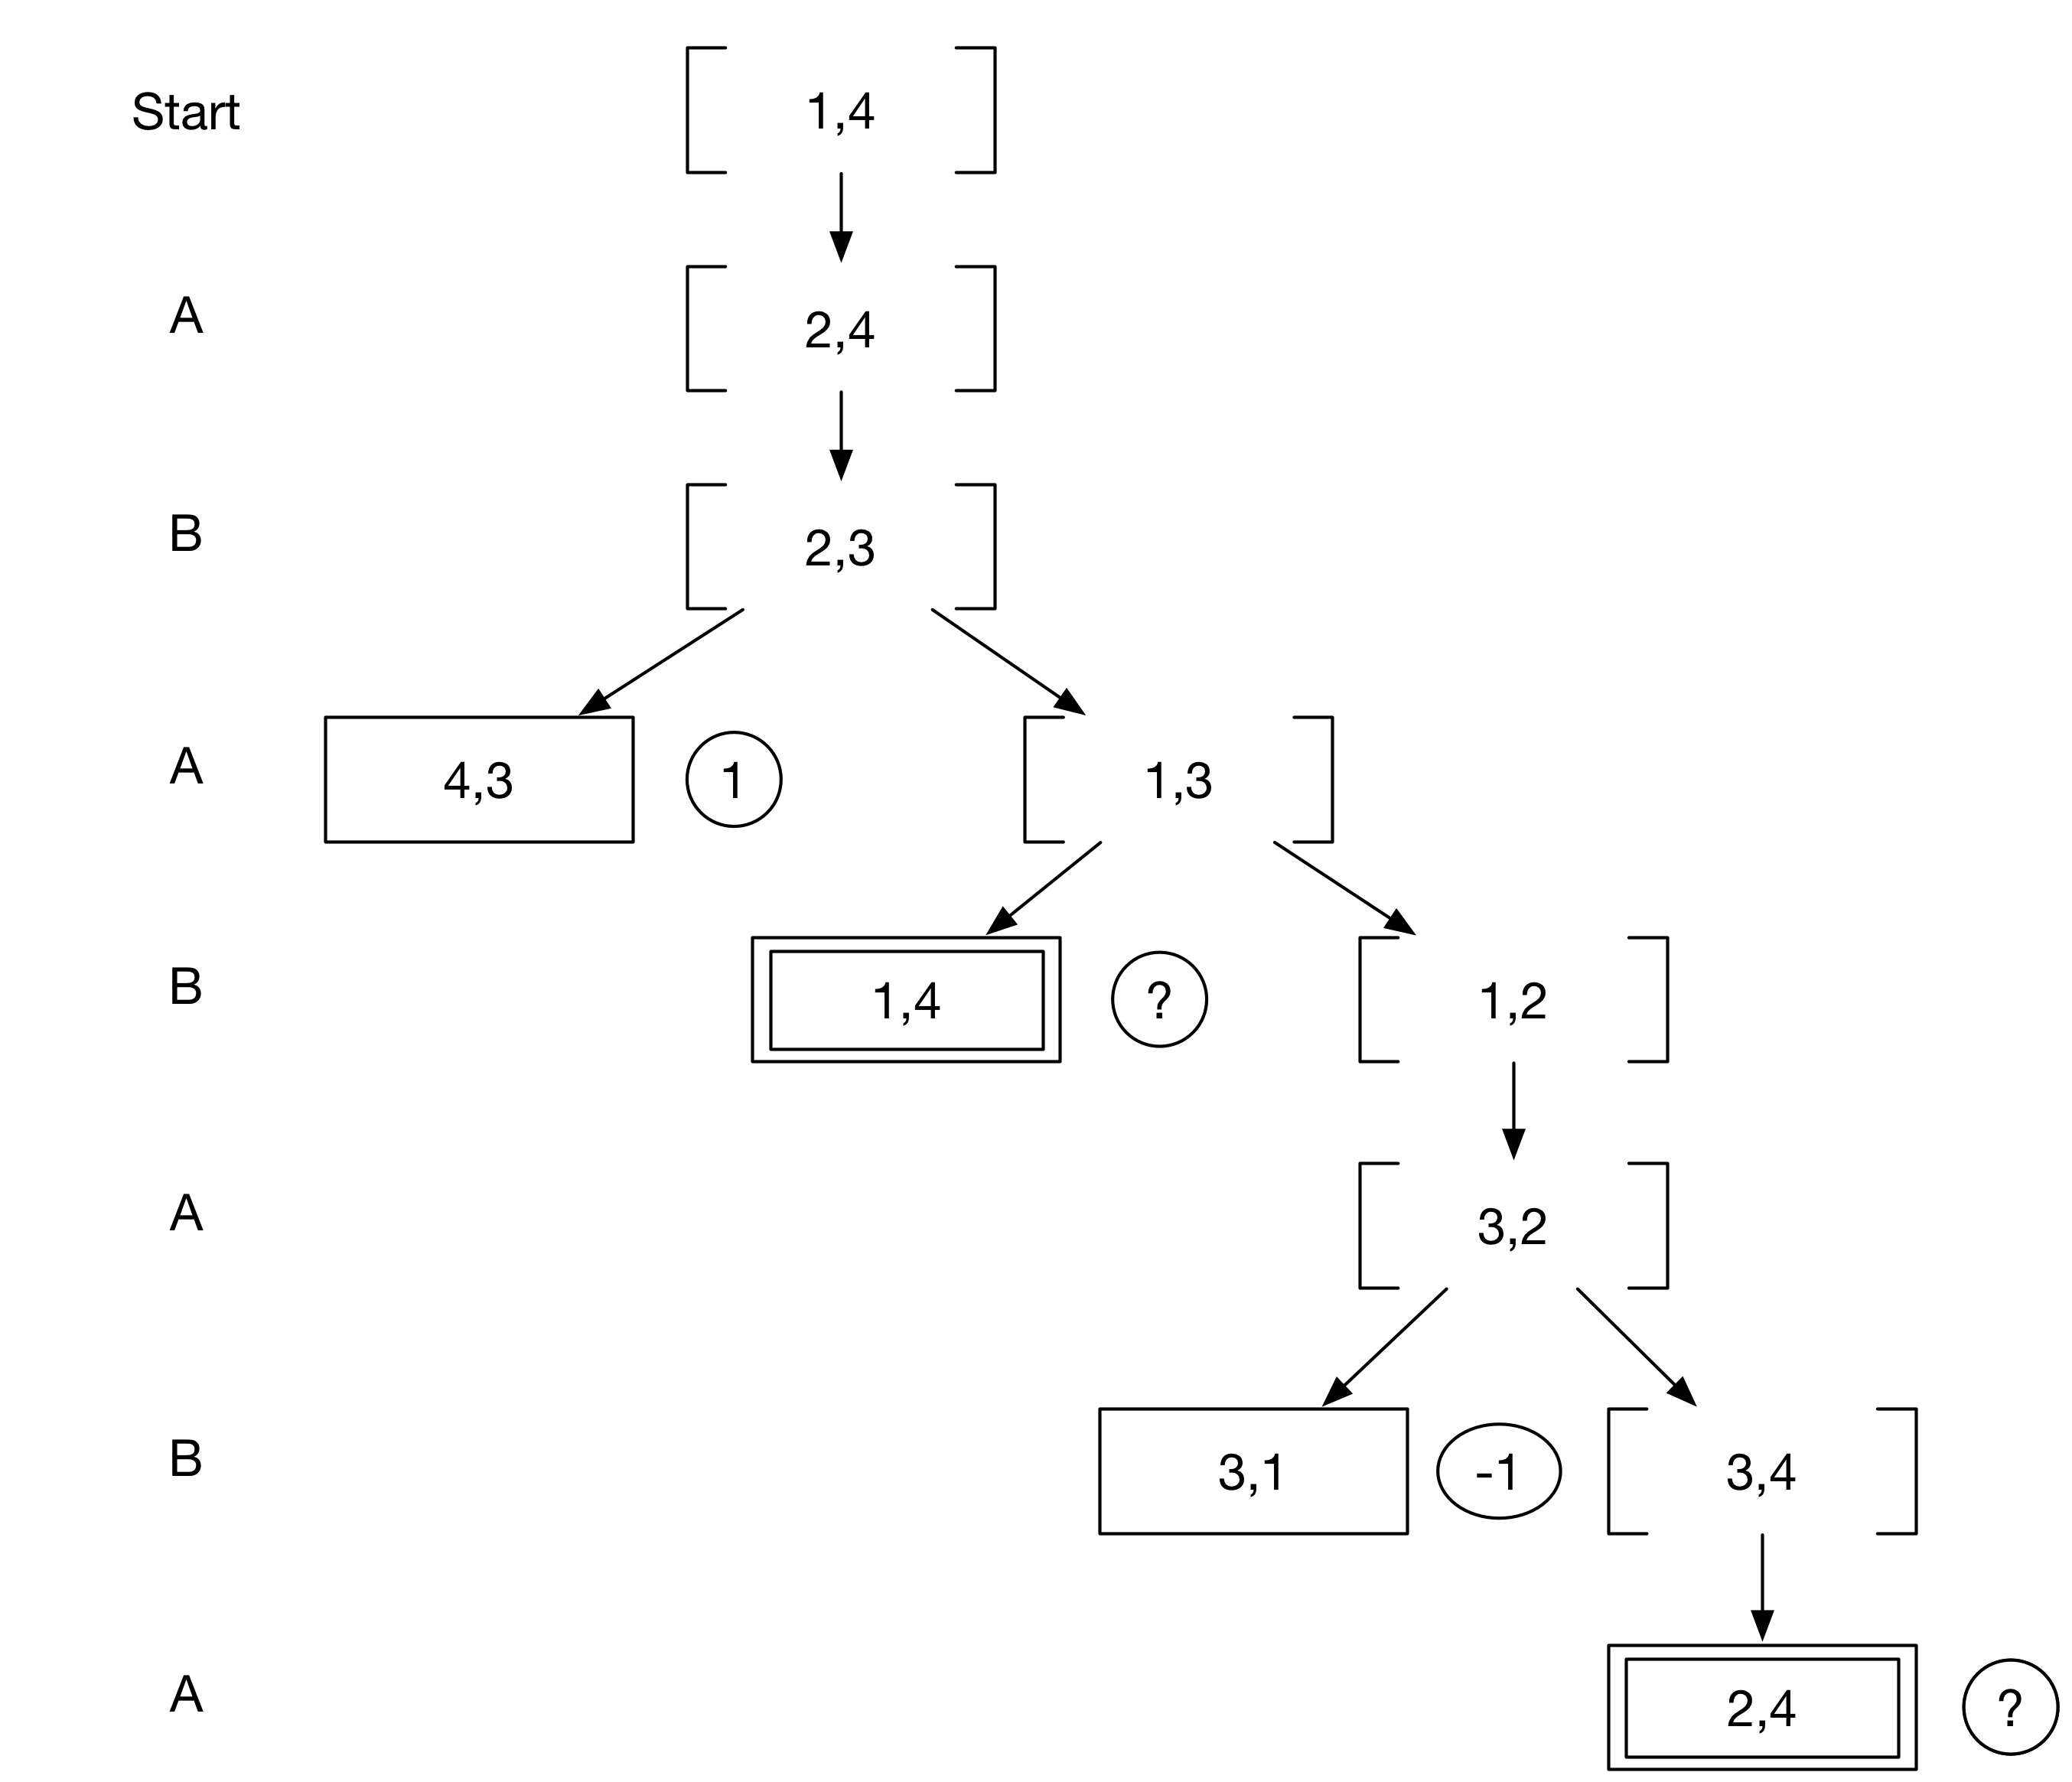
\includegraphics[width=\textwidth]{Problem4a.png}

\newpage
(b)Marked game tree


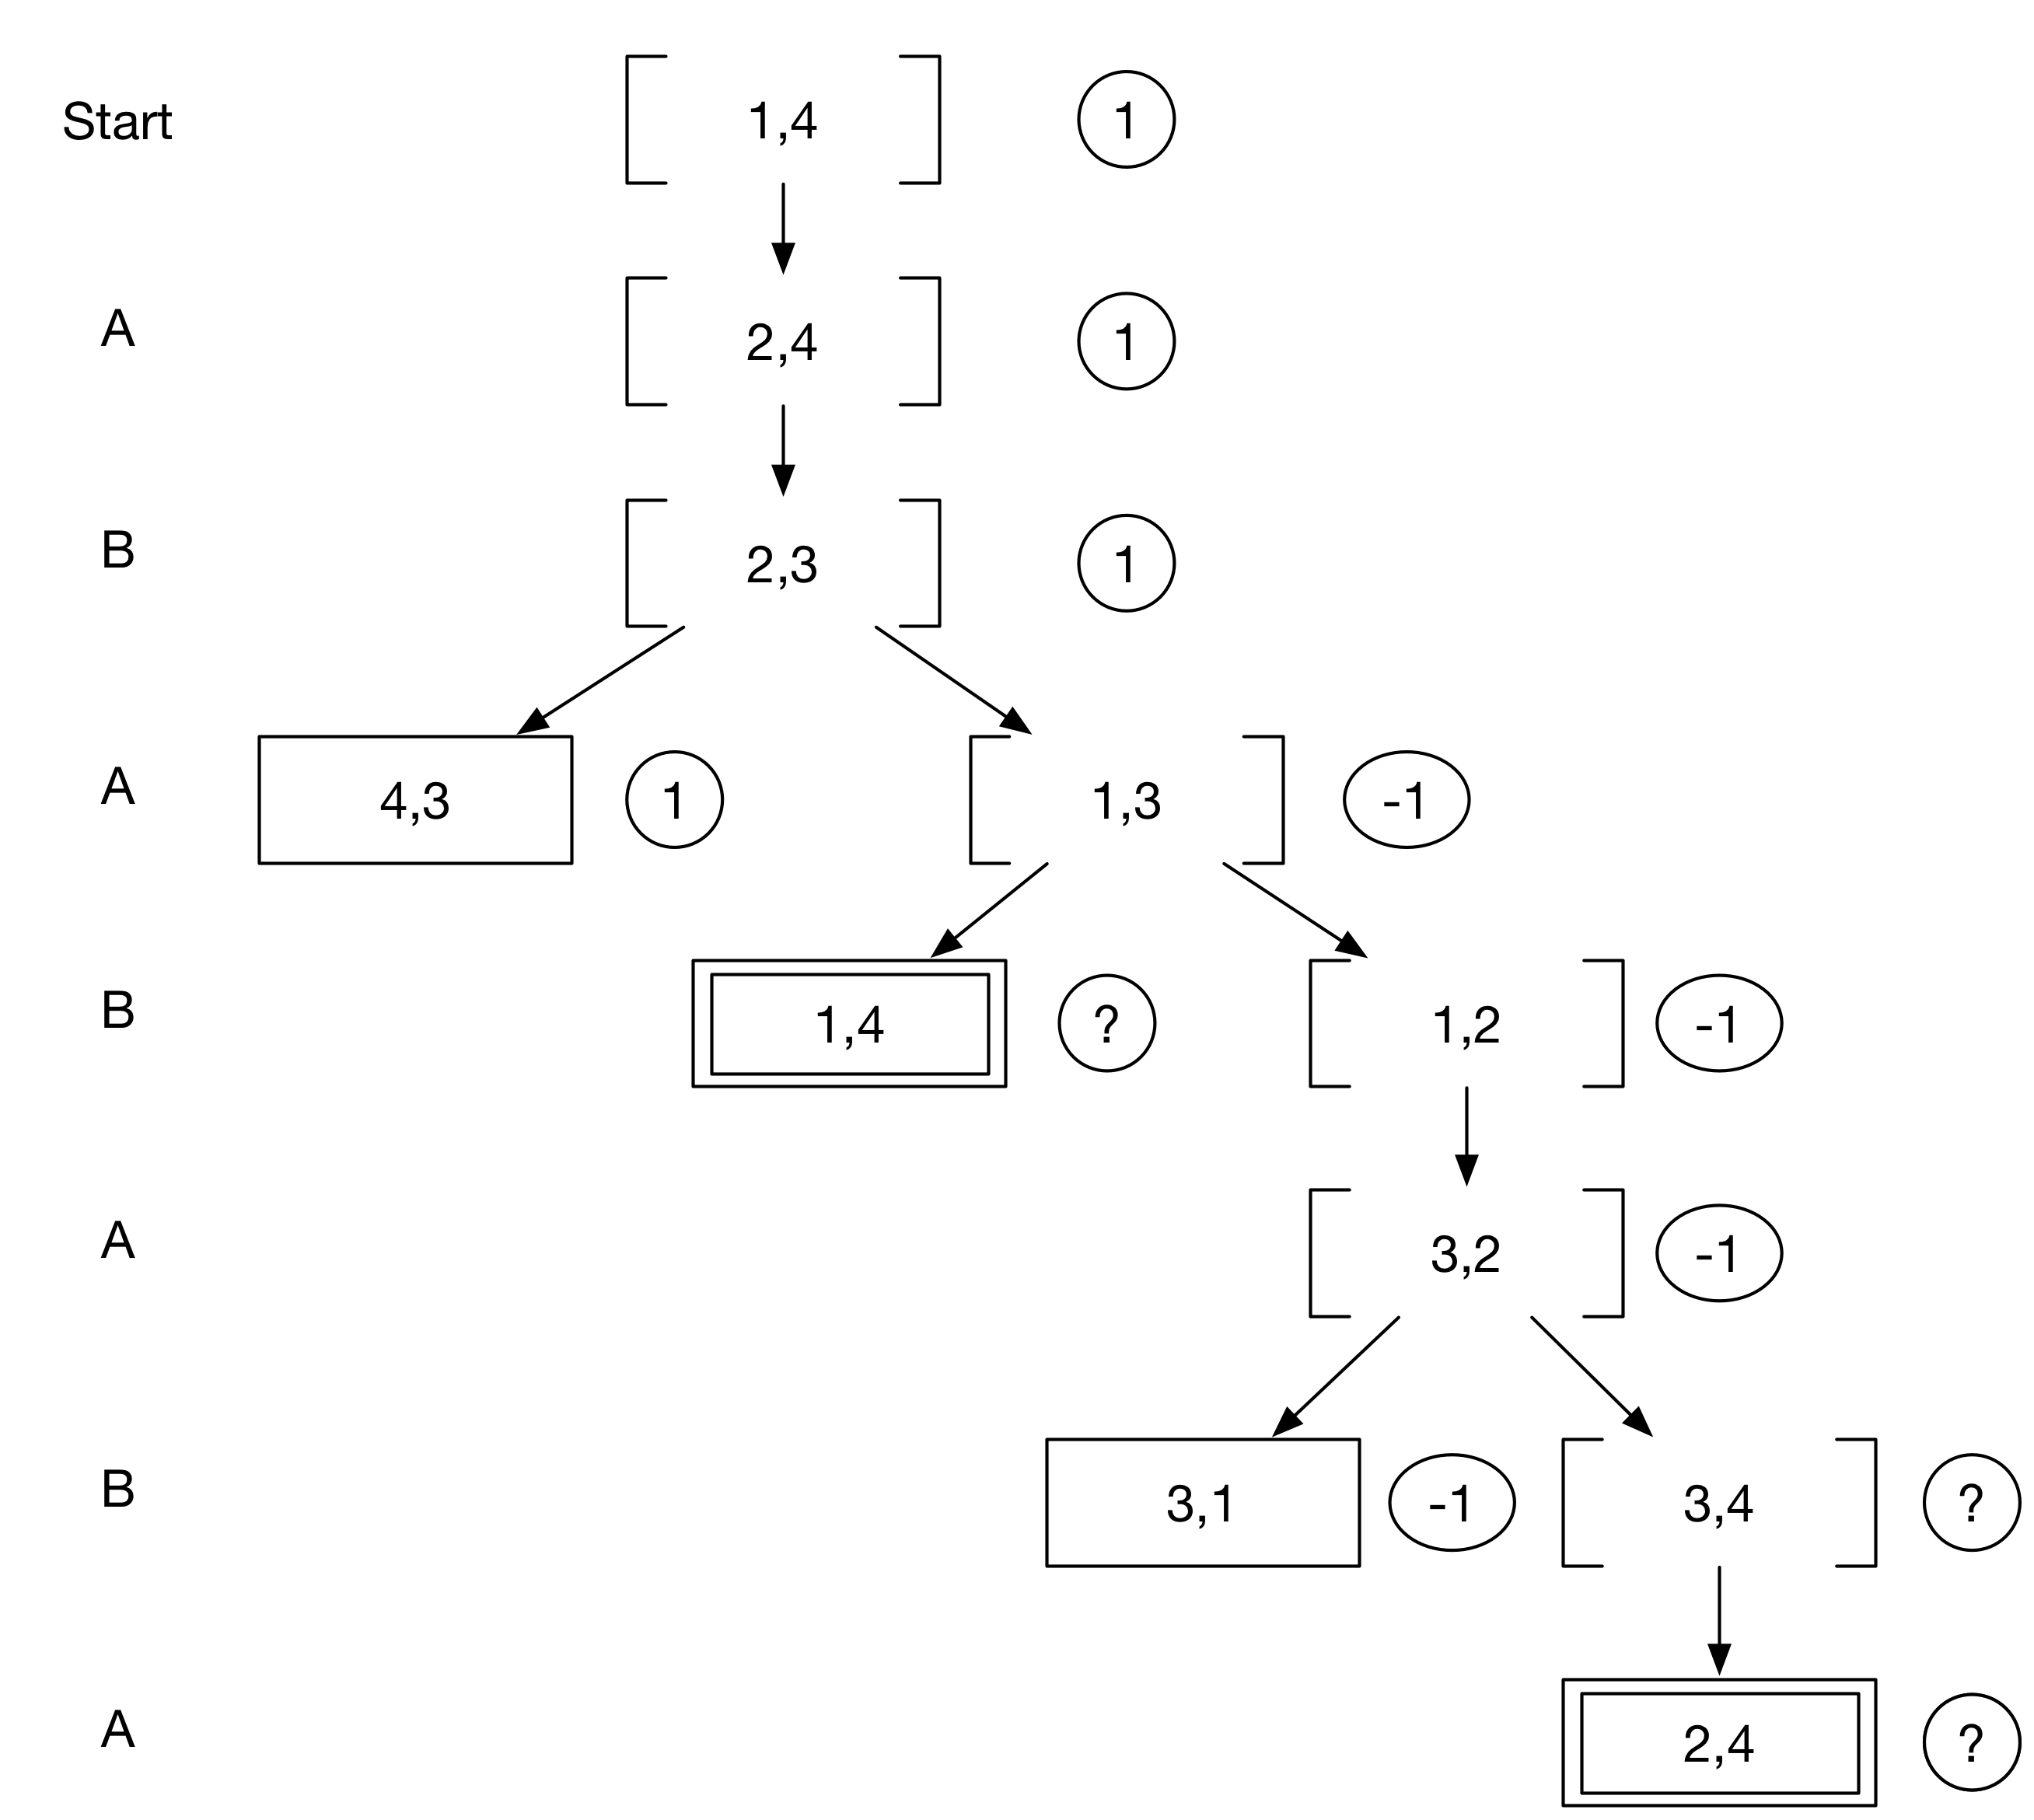
\includegraphics[width=\textwidth]{Problem4b.png}


Decision of B: min(-1,?)=-1, min(?,?)=?

Decision of A: max(1,?)=1, max(?,?)=?

Because in order to win the game, A prefer choosing '1' than '?', B prefer choosing '-1' than '?' as a backed-up value. If two states are both '?', '?' is returned as a backed-up value.


(c)Minimax algorithm failed on this game tree because it runs DFS and meets infinite loop which causes decision tree inifinite. Terminate at the node which has already existed in the tree once, mark it as a loop state and return value '?', handle '?' value with the method mentioned in (b).

If the loop times influences game's value, loop states cannot be denoted as '?', it is a variable and this modified algorithm cannot work at all.

(d)The optimal decision for A and B is constantly going forward, the one that jumps over the other one will win because it moves one more step, so if n is even when A and B meet, A will go across B and A wins, if n is odd, B will go across A and B wins.
\newpage
\section*{Problem 5}
(a)Mark all the nodes 

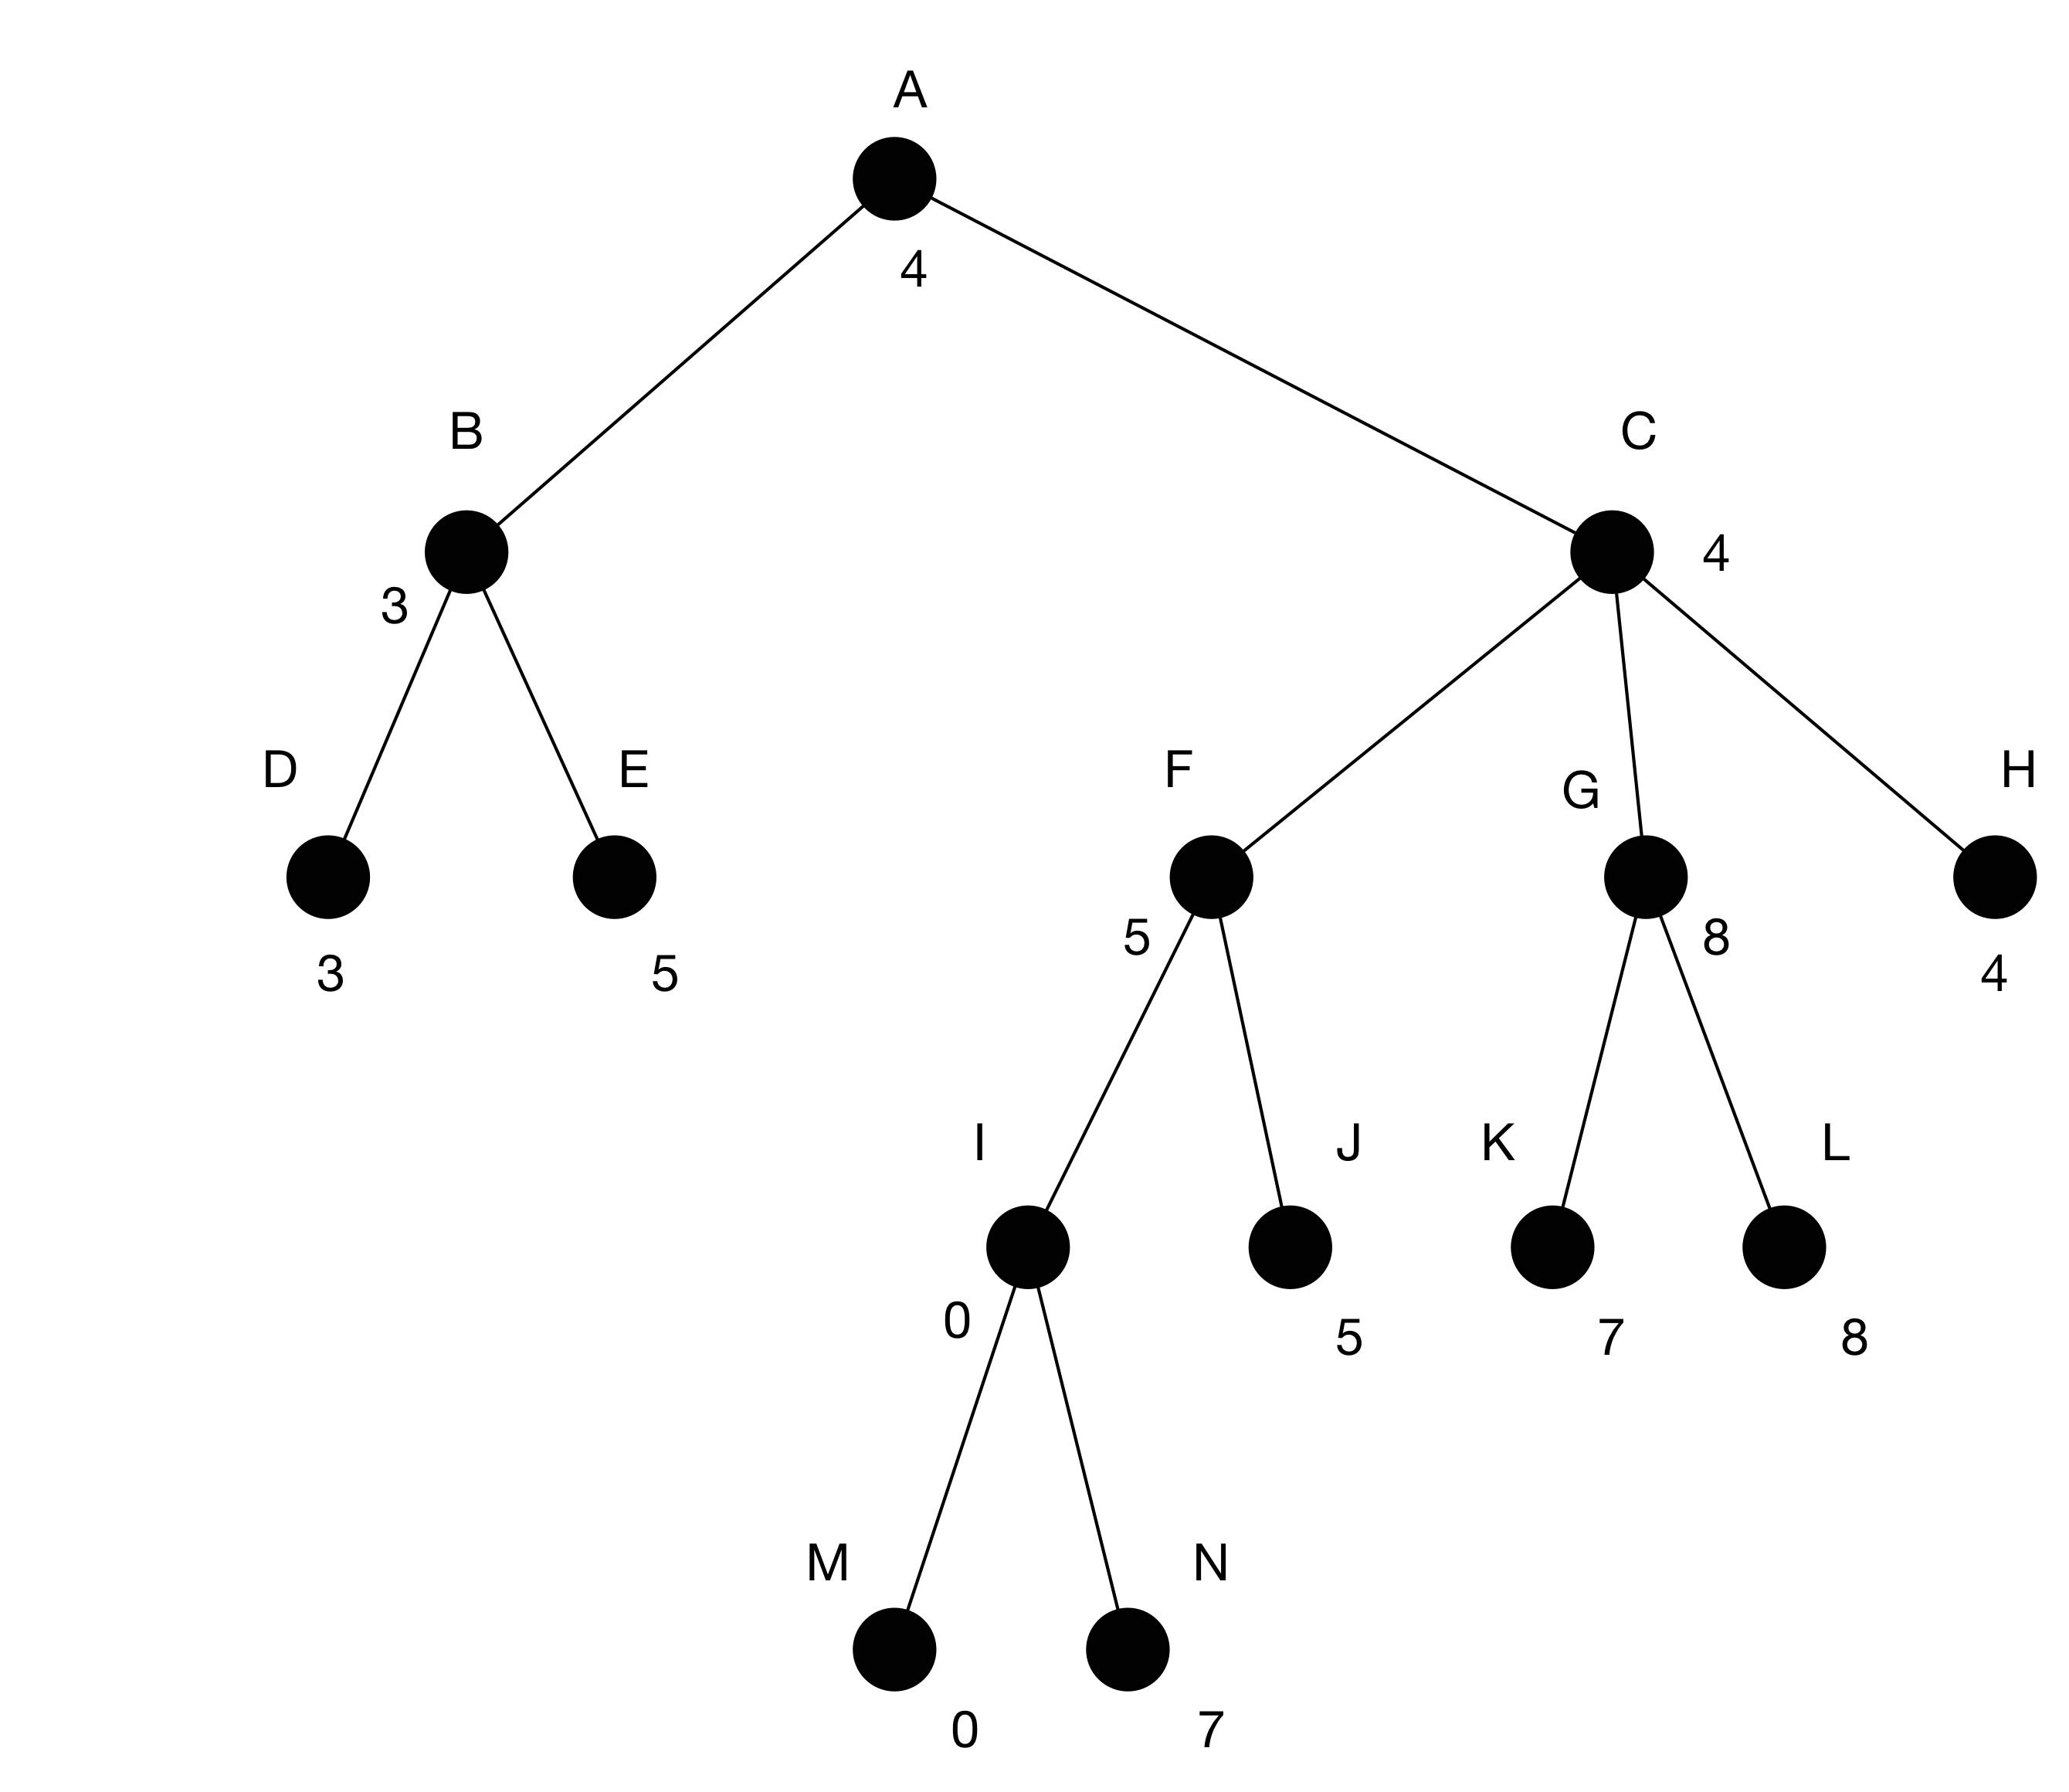
\includegraphics[width=\textwidth]{Problem5a.png}

The best move A $\to$ C, F $\to$ J, G $\to$ L.
\newpage
(2)Nothing changed

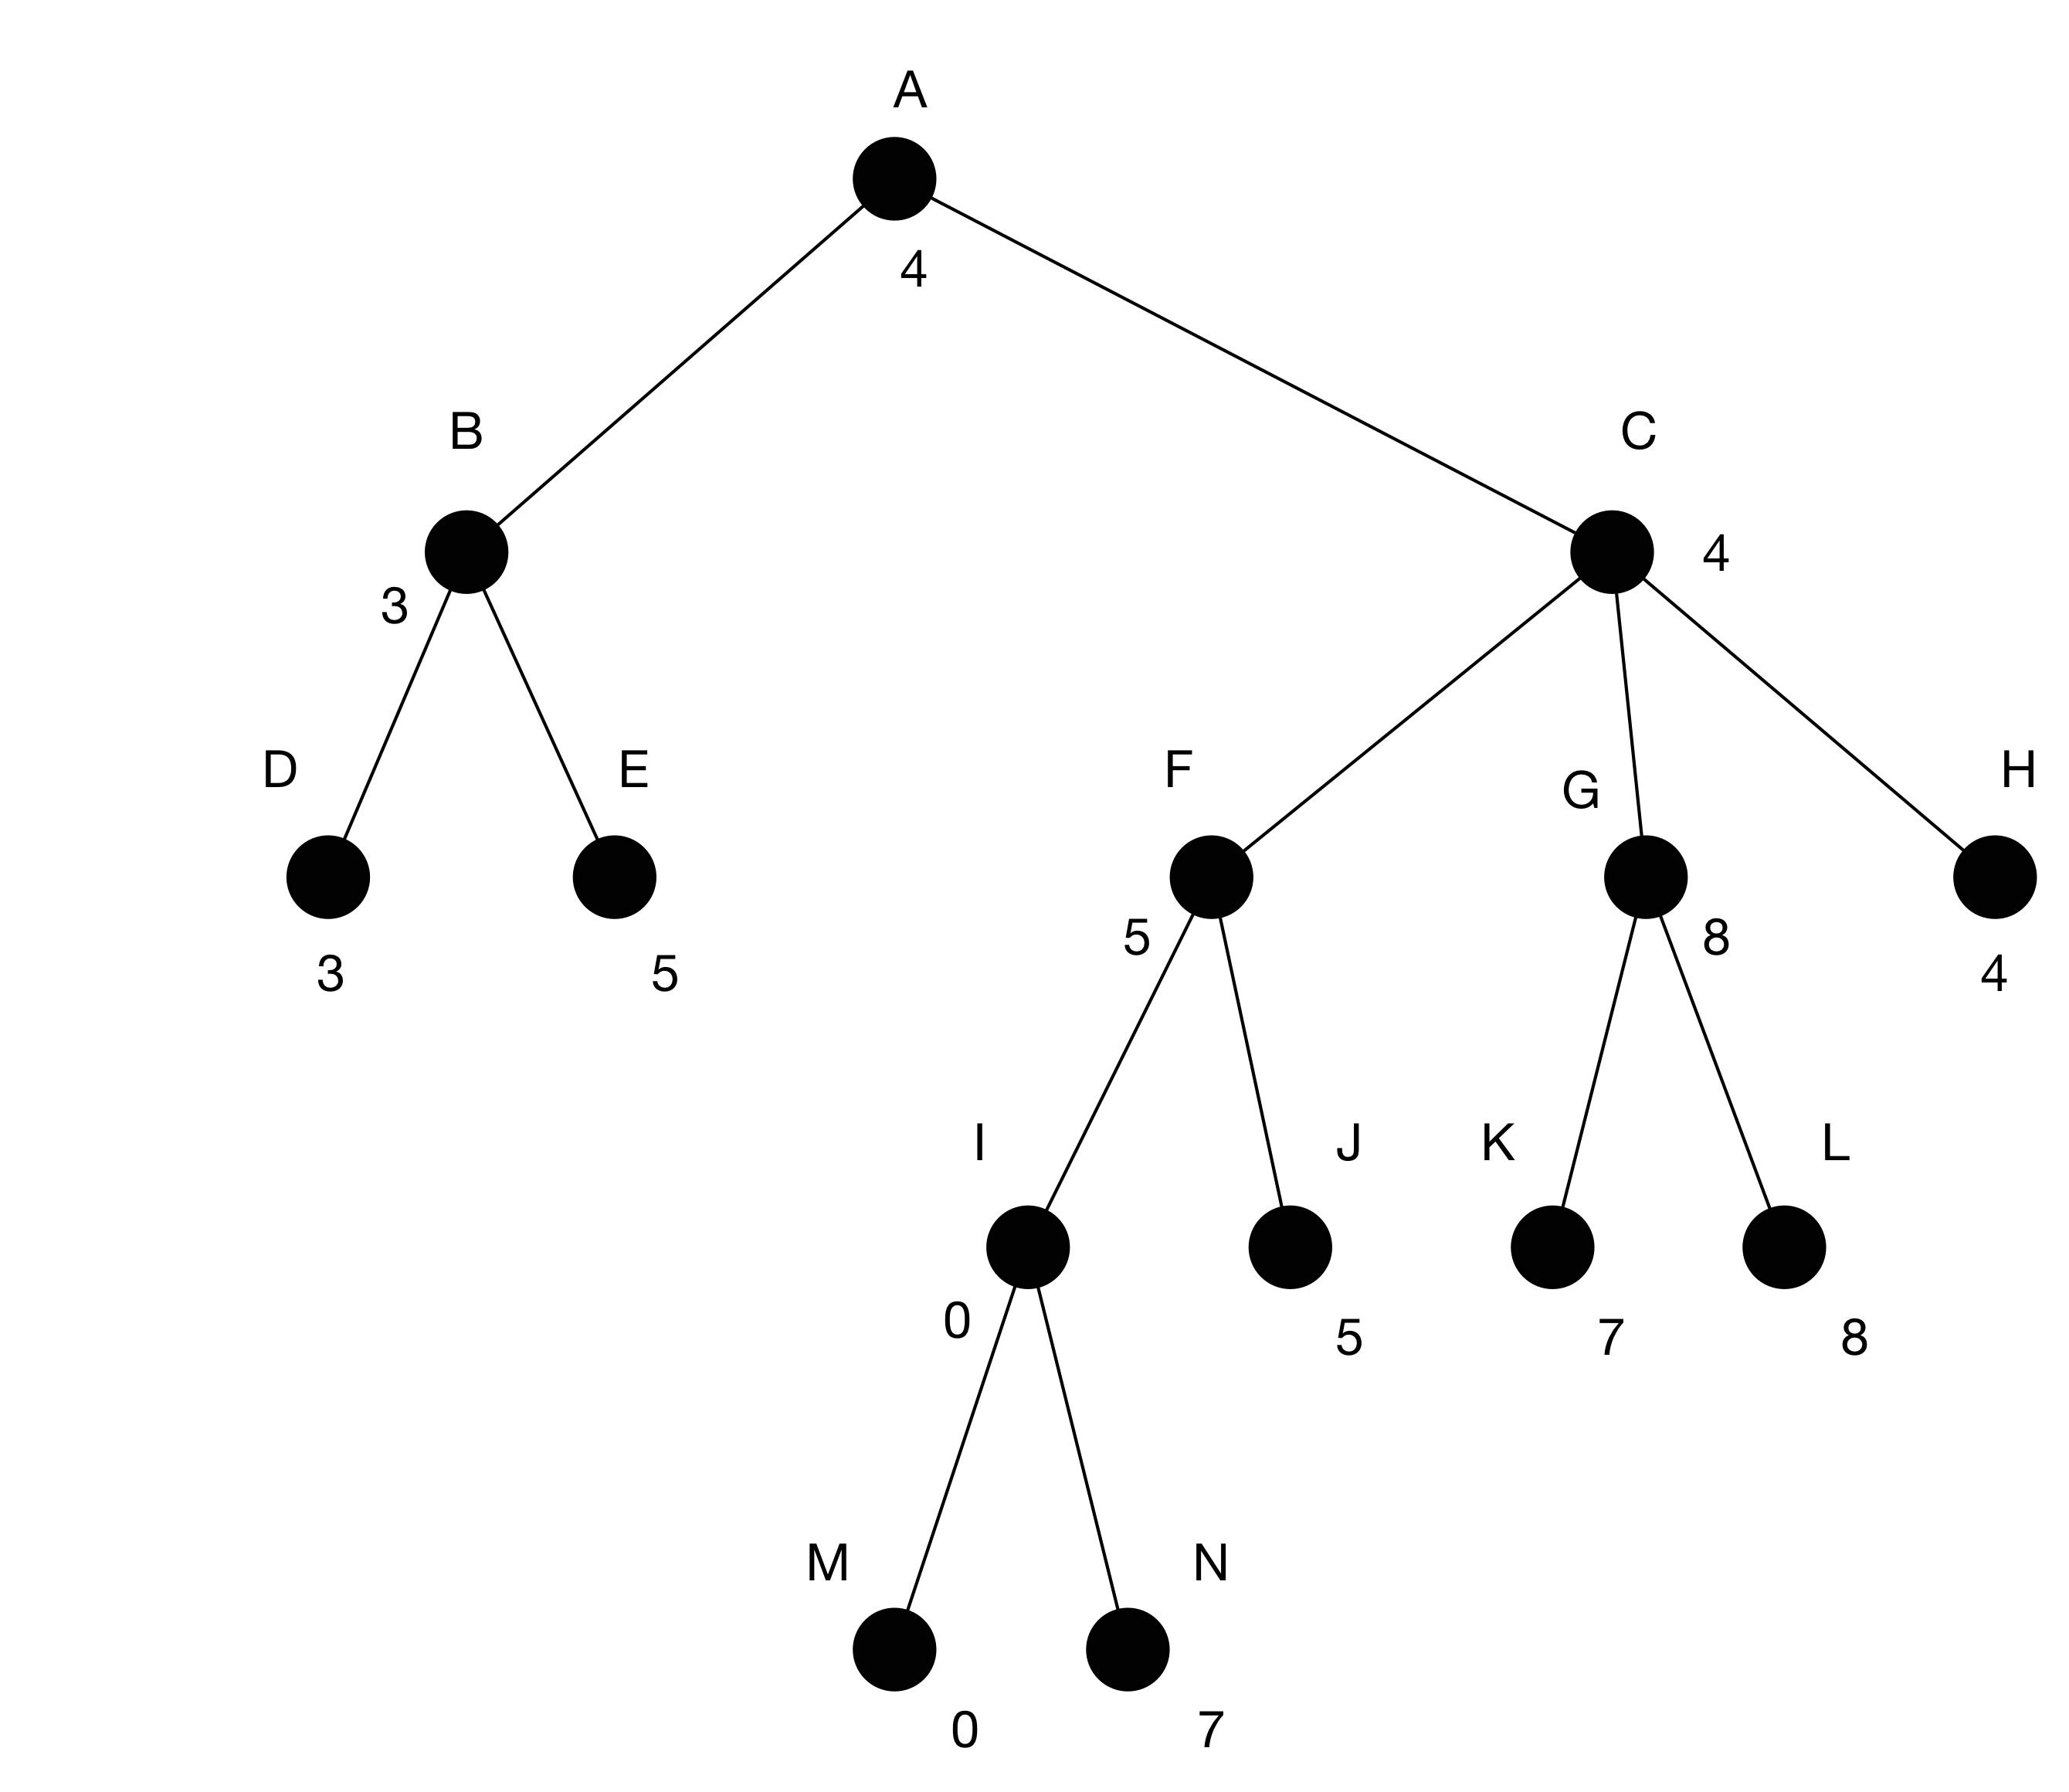
\includegraphics[width=\textwidth]{Problem5b.png}
\newpage
(3)Right-to-left

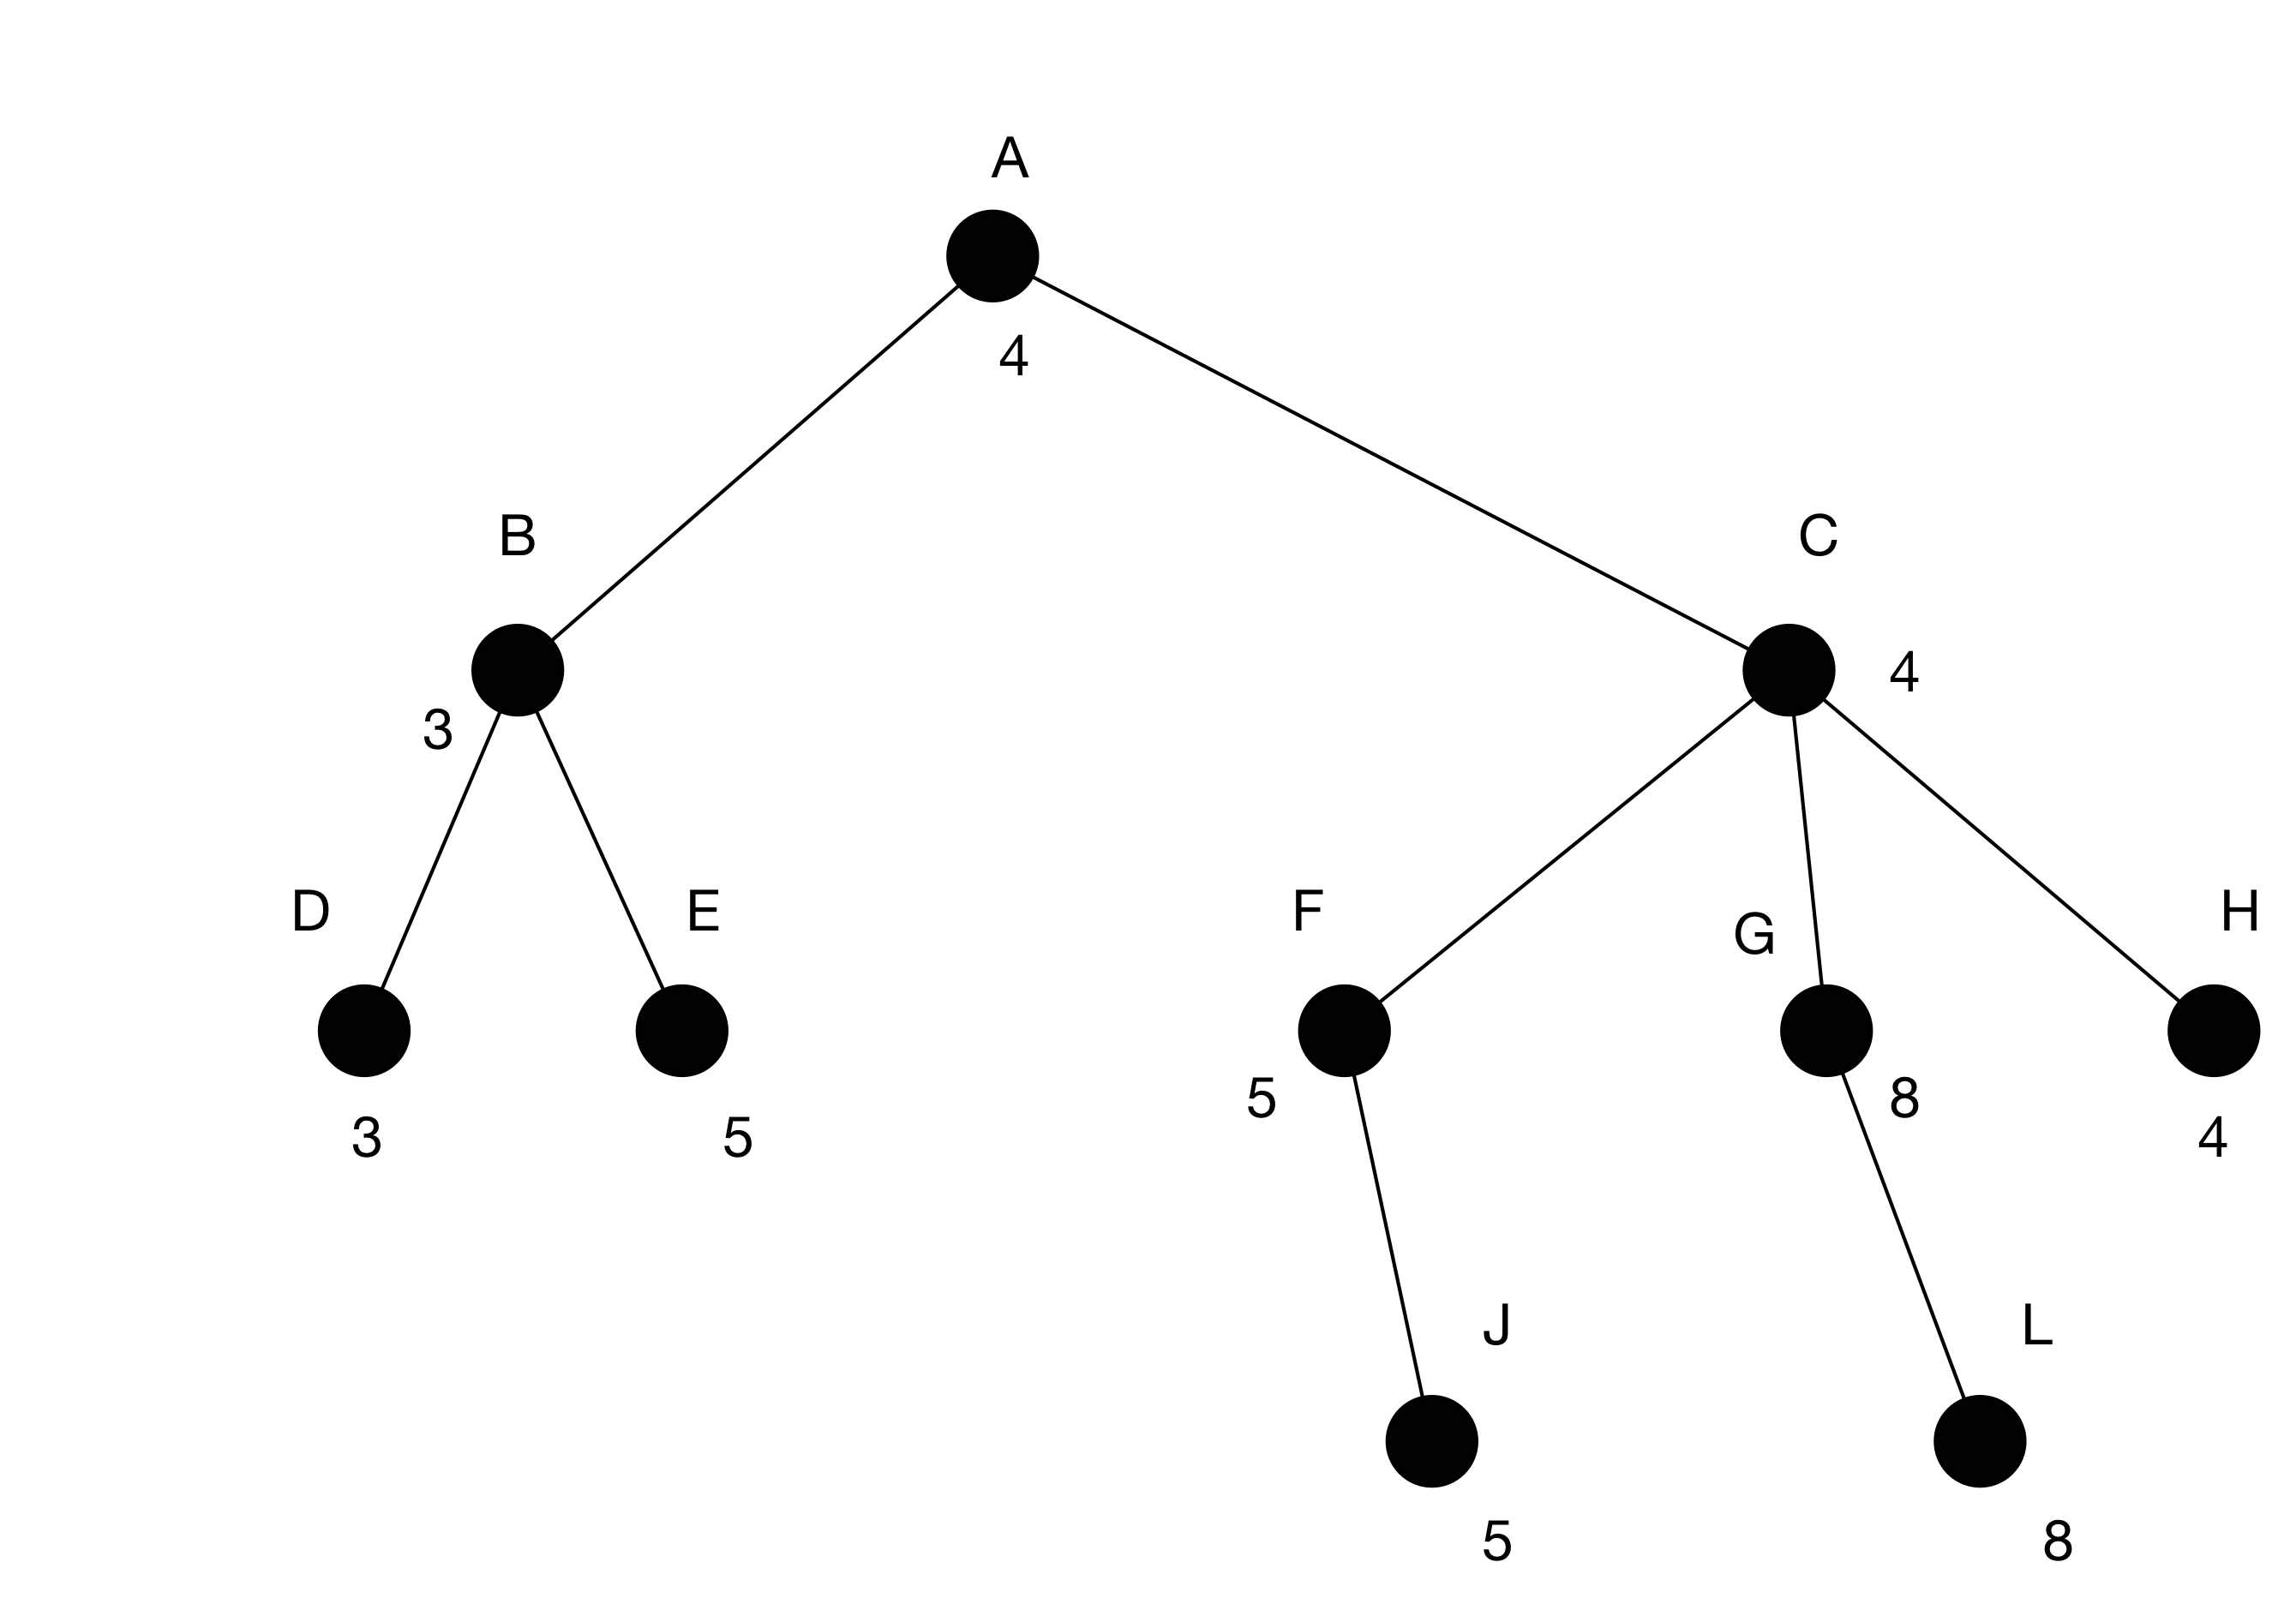
\includegraphics[width=\textwidth]{Problem5c.png}

It is the nodes order that determined search times, \href{https://en.wikipedia.org/wiki/Alpha\%E2\%80\%93beta_pruning}{When nodes are ordered at random, the average number of nodes evaluated is roughly $O(b^{3d/4}) $, If the move ordering for the search is optimal (meaning the best moves are always searched first), the number of leaf node positions evaluated is about $O(b^{d/2})=O({\sqrt {b^{d}}})$.} For example, F $\to$ J will be searched first if it is right-to-left order and F $\to$ I will be abandoned, but if it is left-to-right order, computer needs to completely search F $\to$ I first then finds F $\to$ J.
\newpage


%\iffalse
%\section*{Part 3}
%\subsection*{3.1}
%Repeated Forward A*
%
%
%\subsection*{3.2}
%Repeated Backward A*
%
%
%the results show that Repeated Forward A* and Repeated Backward A* have no significant difference, they have almost the same running time and same expanded number of cells and different paths. The cause of difference of paths is that they have the same break ties rule.
%\section*{Part 4}
%The definition of Manhattan distance: The distance between two points measured along axes at right angles. If the agent only moves in four compass directions, it will only move along the axes we built, it assures that the Manhattan distances are consistent.
%
%It's known that the initial heuristic h is consistent, which means that for any initial state s,  \(h[s] \leq h[s_{succ}] + c(s, a)\) . This inequality will hold for all non-goal state s and their corresponding actions. if some action costs c(s, a) increases from c to c', and $c(s, a) \leq c'(s, a)$,   \(h[s] \leq h[s_{succ}] + c(s, a) \leq h[s_{succ}] + c'(s, a)\) , the heuristic remain consistent. The heuristic function h of state s become $h_{new}$,  $(h_{new}) = g[\bar{s}] + h[\bar{s}]  - g[s]$ and expansion. They, we can divide s into the following situations.
%
%\begin{enumerate}
%\item both s and succ(s, a) were expanded.  $(h_{new}[s]) = g[\bar{s}] + h[\bar{s}]  - g[s]$ $(h_{new}[succ(s, a)]) = g[\bar{s}] + h[\bar{s}]  - g[succ(s, a)]$, according to triangle inequality,  $ g[succ(s, a)] \leq g(s) + c(s, a)$, 
%$(h_{new}[s]) = g[\bar{s}] + h[\bar{s}] - g[s] \leq  g[\bar{s}] + h[\bar{s}] - (g[succ(s, a)] - c(s, a)$. thus $(h_{new}[s]) \leq (h_{new}[succ(s, a)]) + c(s, a)$
%\item 
%s were expanded but succ(s, a) were not expanded, $(h_{new}[s]) = g[\bar{s}] + h[\bar{s}]  - g[s]$ , $g[\bar{s}] + h[\bar{s}] \leq f[succ(s, a)]$,  $h_{new}[s] = g[\bar{s}] + h[\bar{s}]  - g[s] \leq g[succ(s, a)] + h'_{new}[succ(s, a)] -g[succ(s, a)] + c[s, a] \leq h'_{new}[succ(s, a)] +  c[s, a] $
%\item 
%both s and succ(s, a) were not expanded, $then h[s] \leq h[(succ(s, a))] + c(s, a)$
%\end{enumerate}
%\newpage
%\section*{Part 5}
%\subsection*{5.1}
%Repeated Forward A*
%
%
%\subsection*{5.2}
%Adaptive A*
%
%
%the results show that Adaptive A* expanded fewer cells than Repeated Forward A* and has less running time if the path is short enough.
%\newpage
%\section*{Part 6}
%The tree pointer can be represented as a two bit number .
%\begin{lstlisting}
%val directions = List((0, 1), (0, -1), (1, 0), (-1, 0))
%\end{lstlisting}
%It is calculated by father node coordinate minus child node coordinate.
%
%Another way is to use sparse matrix representing the maze since the quantity of blocked cells is small enough.
%\begin{lstlisting}
%sys.getsizeof(grid.array)
%10313
%\end{lstlisting}
%Python implementation of a 2-d array gridworld takes 10313 Bytes
%\begin{lstlisting}
%array = sparse.csr_matrix(array)
%sys.getsizeof(grid.array[0])
%64
%\end{lstlisting}
%Compressed Sparse Row method can be found in \emph{scipy} libray. 106 gridworlds can be stored in 4 MBytes using 2-d array.
%If gridworld is 1001*1001, it is approximately 13 gridworlds can be stored in 4 MBytes using sparse matrix.
%\fi


\end{document}